\begin{appendix} 

\section{TMC4671}\label{Appendix:TMC4671}

\subsection{Standard-Schaltkreis TMC4671}

\begin{figure}[h!]
	\centering
	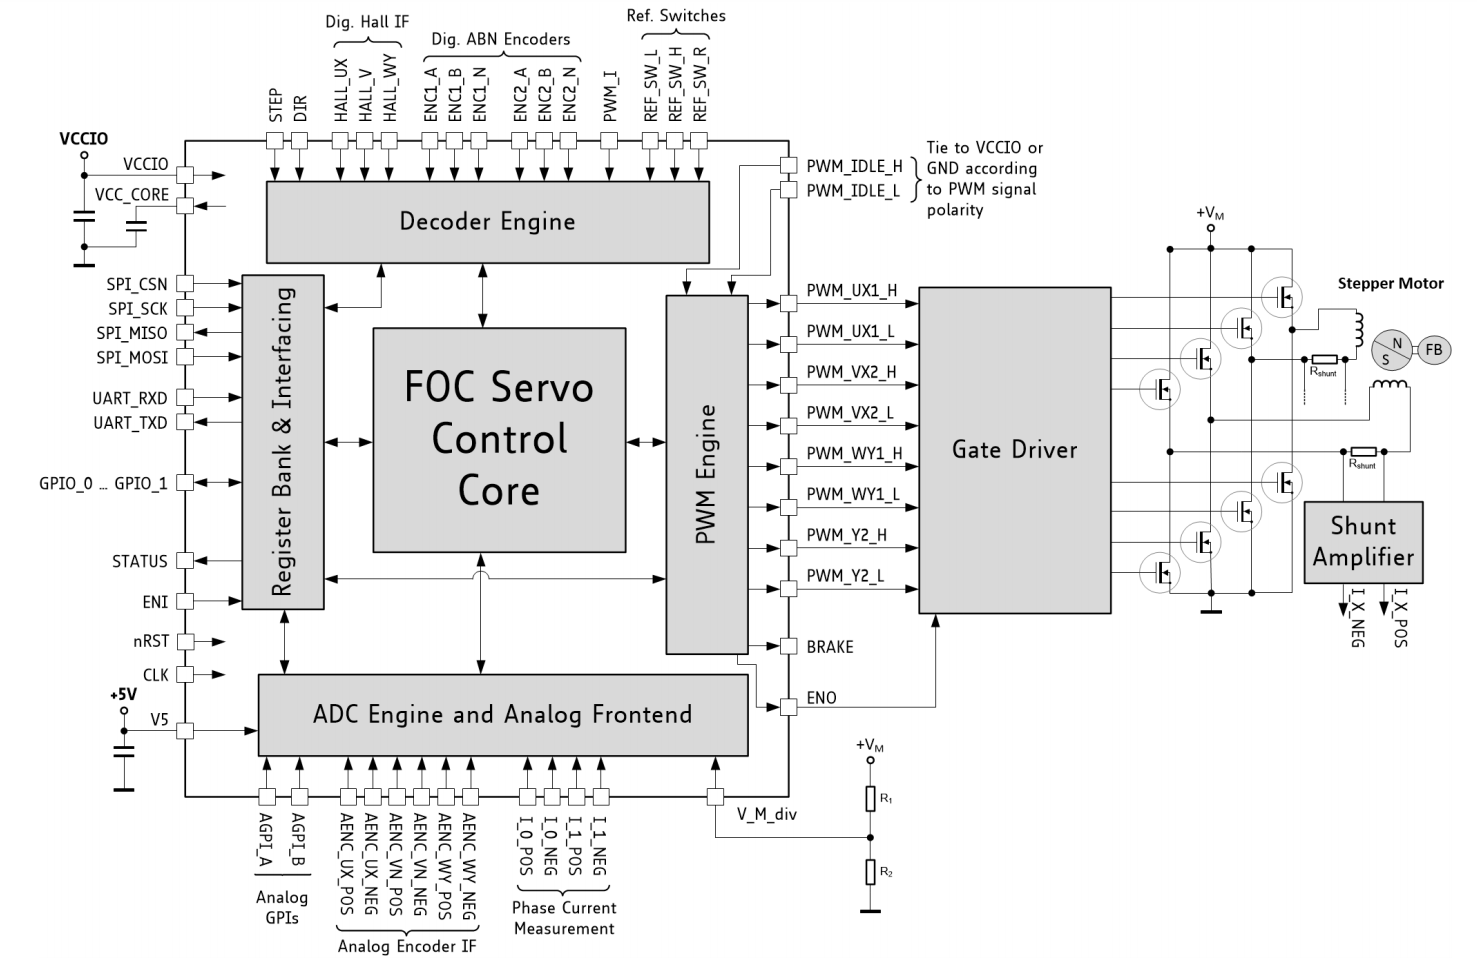
\includegraphics[width=0.8\textwidth]{graphics/Standard_Application_Cirquit_TMC4671}
	\caption{Standard-Anwendungs-Schaltung.}
	\label{fig:Schaltung_TMC4671}
\end{figure}
\todo{cite{TMC4671 Datenblatt}}

\subsection{Blockdiagramm TMC4671}

\begin{figure}[h!]
	\centering
	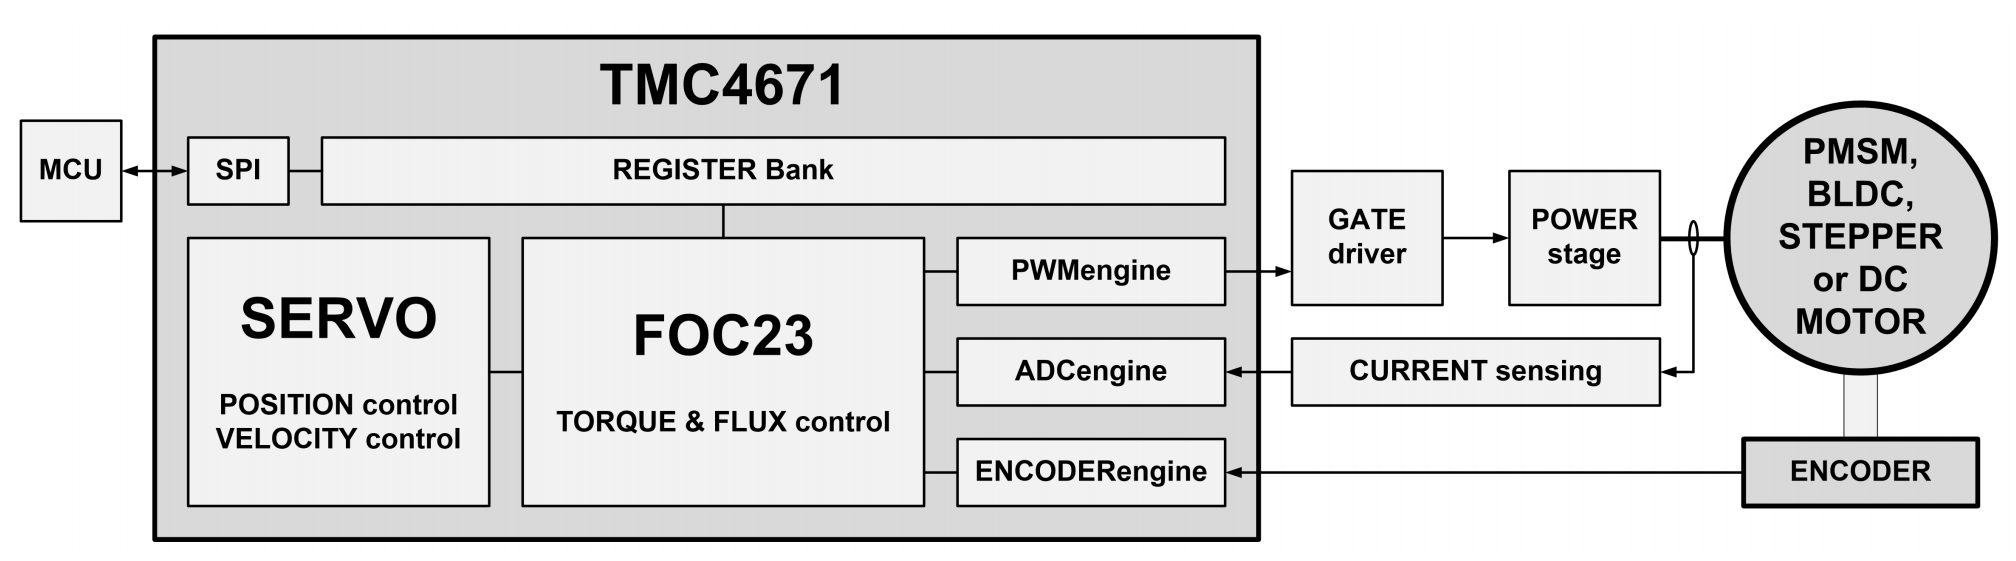
\includegraphics[width=0.8\textwidth]{graphics/Blockdiagramm_TMC4671}
	\caption{Blockdiagramm TMC4671.}
	\label{fig:Blockdiagramm_TMC4671}
\end{figure}
\todo{cite{TMC4671 Datenblatt}}

\newpage

\section{TMC6200}\label{Appendix:TMC6200}

\subsection{Standard-Schaltkreis TMC6200}

\begin{figure}[h!]
	\centering
	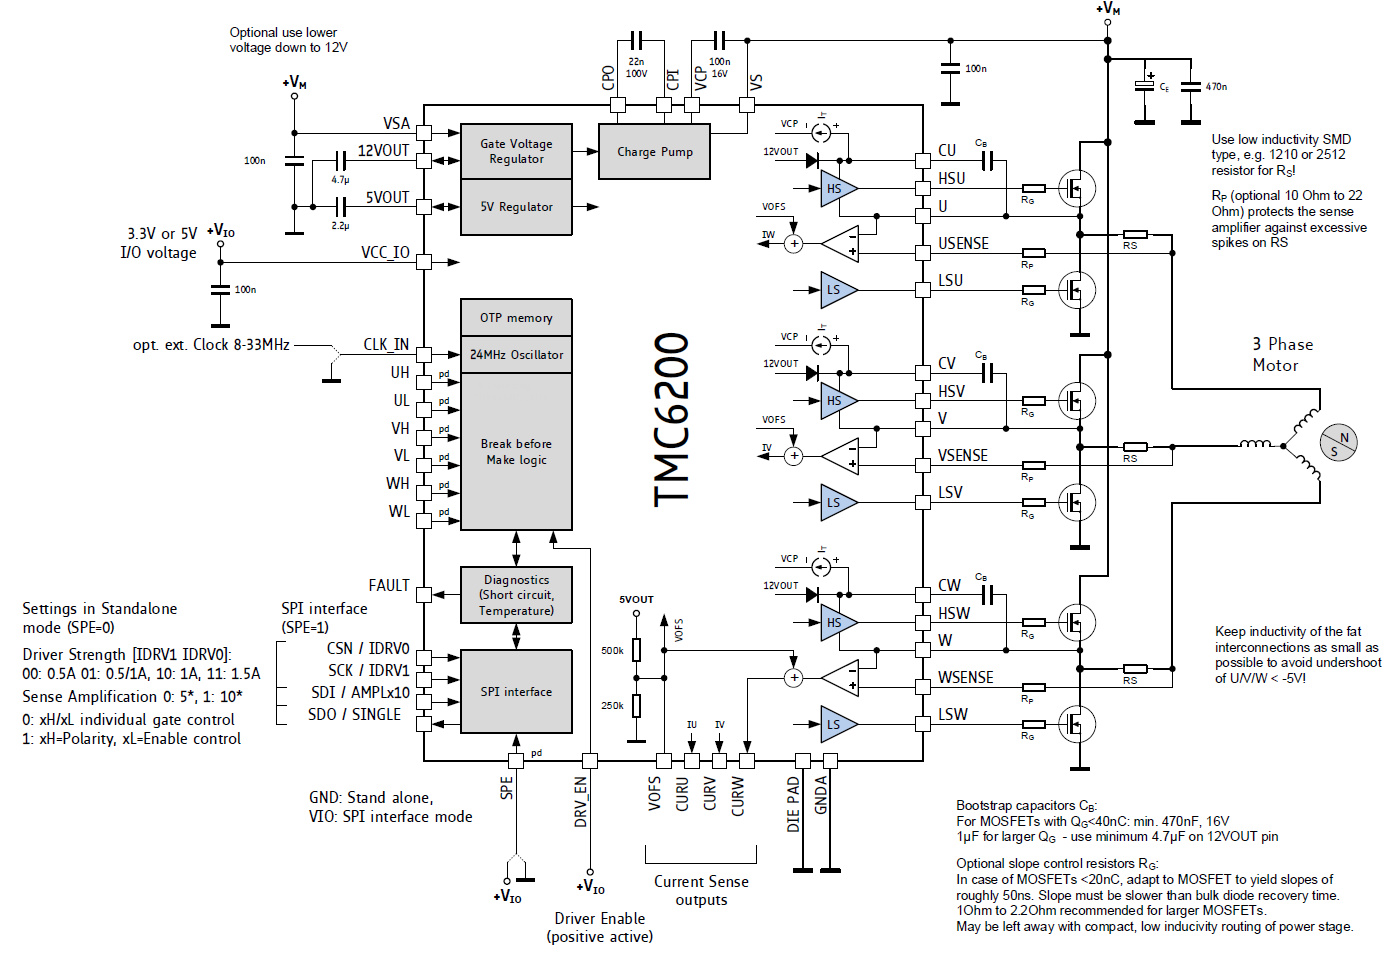
\includegraphics[width=0.8\textwidth]{graphics/Standard_Application_Cirquit_TMC6200.png}
	\caption{Standard-Anwendungs-Schaltung TMC6200.}
	\label{fig:Schaltung_TMC6200}
\end{figure}

\subsection{Blockdiagramm TMC6200}

\begin{figure}[h!]
	\centering
	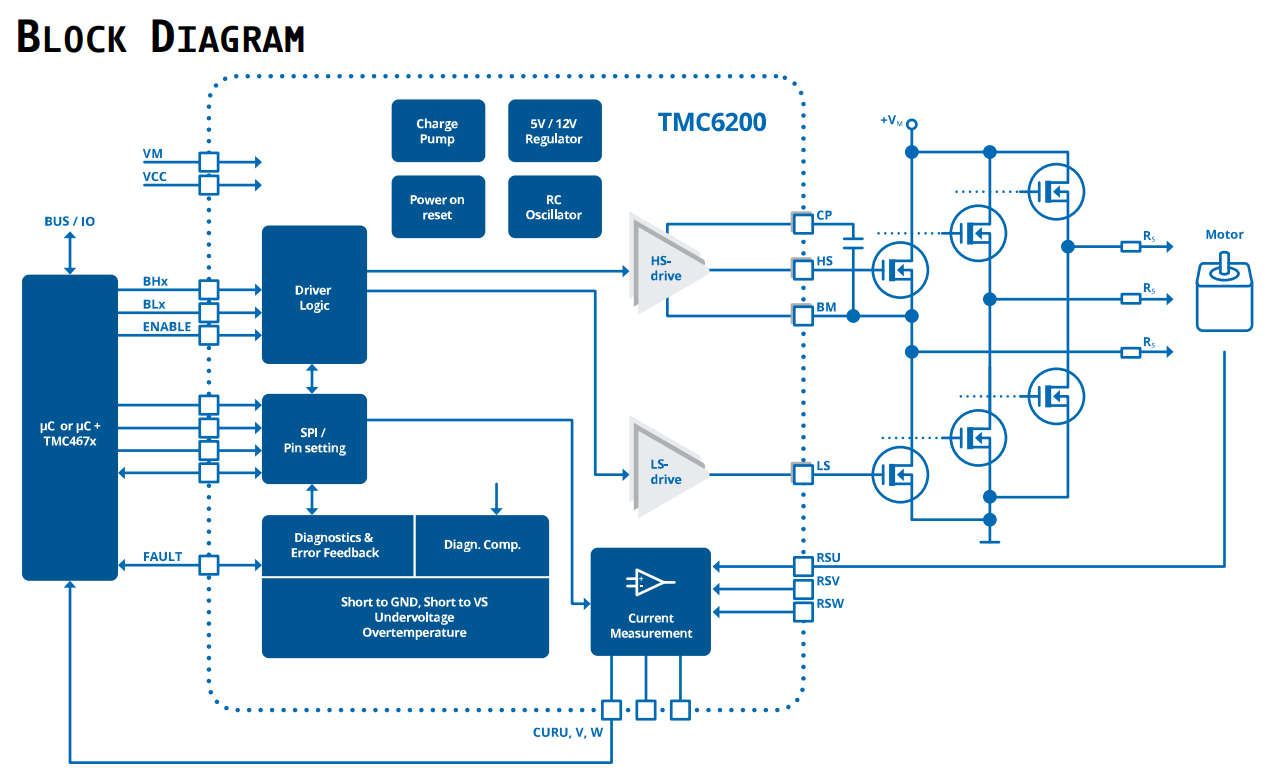
\includegraphics[width=0.8\textwidth]{graphics/Blockdiagramm_TMC6200.png}
	\caption{Blockdiagramm TMC6200.}
	\label{fig:Blockdiagramm_TMC6200}
\end{figure}

\newpage

\subsection{Verstärkungsfaktor, Strommessung, Strommesswiderstand}

\begin{figure}[h!]
	\centering
	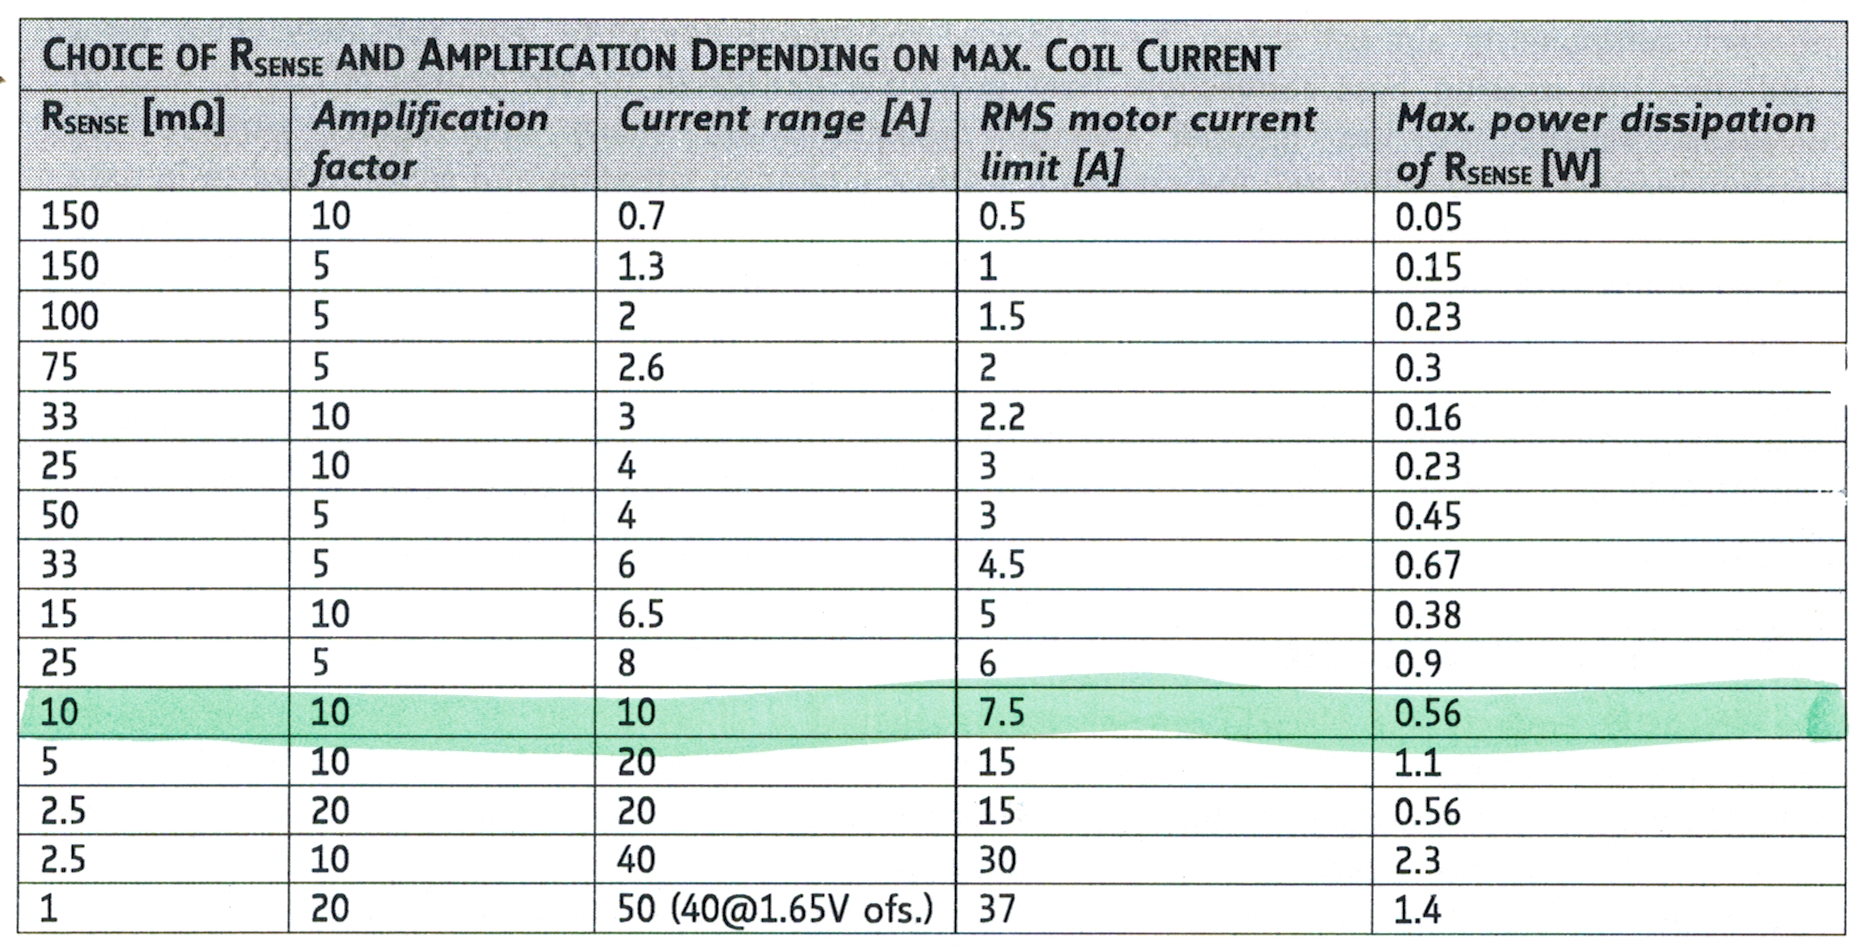
\includegraphics[width=\textwidth]{graphics/Tabelle_Shunts.png}
	\caption{Tabelle zur Bestimmung des Strommesswiderstandes aus dem Datenblatt von Trinamic.}
	\label{fig:Tabelle_Shunts}
\end{figure}

\subsection{Gate-Vorwiderstand}

\begin{figure}[h!]
	\centering
	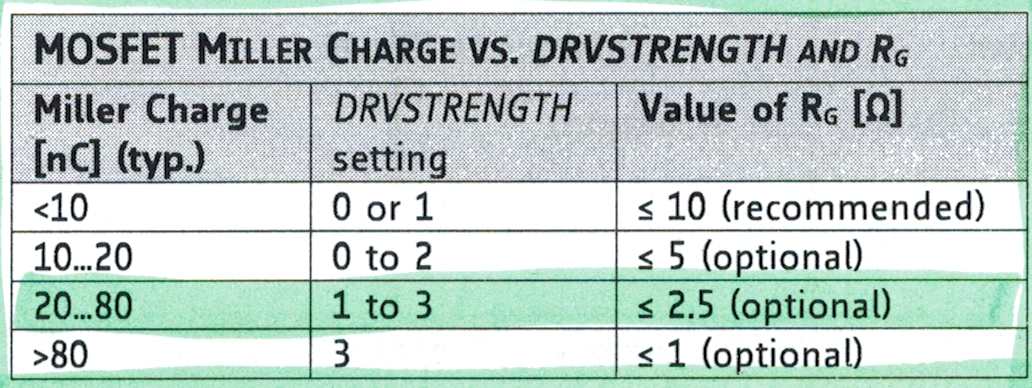
\includegraphics[width=0.5\textwidth]{graphics/Tabelle_Gatewiderstaende.png}
	\caption{Tabelle zur Bestimmung der Gatewiderstände aus dem Datenblatt von Trinamic.}
	\label{fig:Tabelle_Gatewiderstaende}
\end{figure}

\subsection{Externe Gate-Spannungsversorgung}

\begin{figure}[h!]
	\centering
	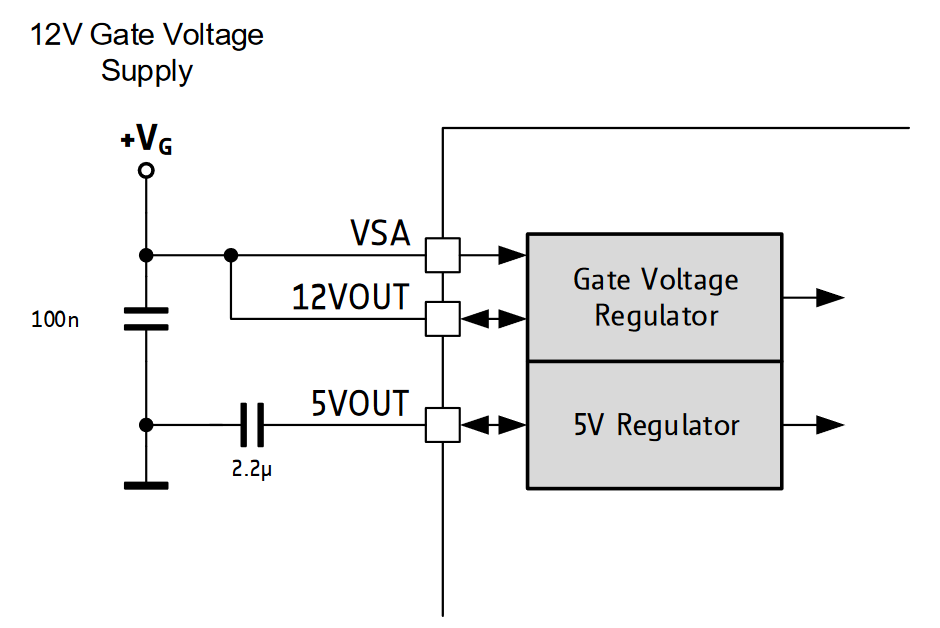
\includegraphics[width=0.5\textwidth]{graphics/Schema_Gate_Treiber_Gatespannung}
	\caption{Schema externe Gate-Spannungsversorgung.}
	\label{fig:Schema_Gate_Treiber_Gatespannung}
\end{figure}

\newpage

\section{H-Brücke}\label{Appendix:H_Bruecke}

\subsection{Referenzschema}

\begin{figure}[h!]
	\centering
	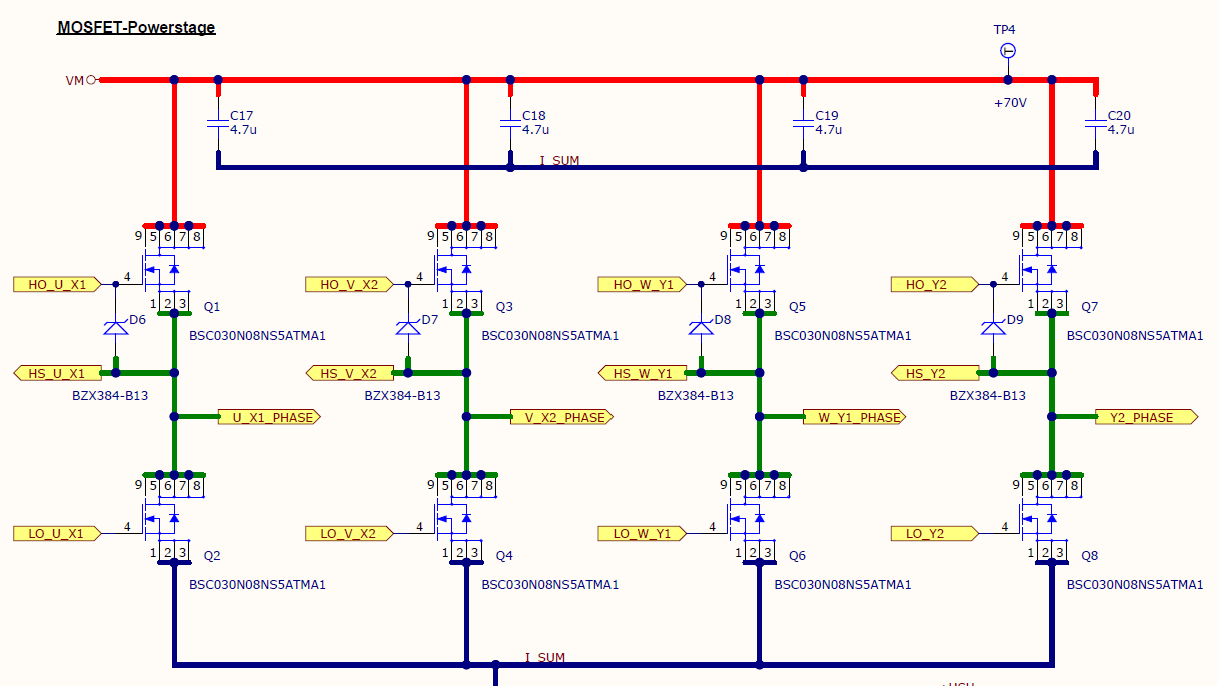
\includegraphics[width=0.7\textwidth]{graphics/Referenzschema_10A70V}
	\caption{H-Brücke.}
	\label{fig:Schema_H_Bruecke_und_BLDC_Ref}
\end{figure}

\todo{cite: Datenblatt UPS 10A70V Schema}

\section{Mikrocontroller}\label{Appendix:Mikrocontroller}

\subsection{Brown-out-Detection}\label{Appendix:Brown-out-Detection}

\begin{figure}[h!]
	\centering
	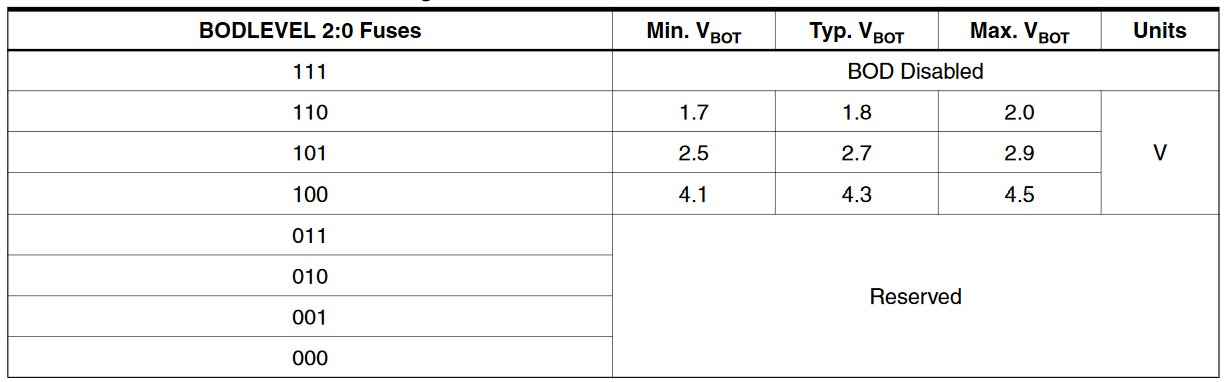
\includegraphics[width=0.7\textwidth]{graphics/Tabelle_BoD}
	\caption{Tabelle Brown-out-Detection.}
	\label{fig:Tabelle_BoD}
\end{figure}

\todo{cite: Datenblatt Atmega 2560, Seite 361}

\subsection{Full Swing Crystal Oscillator}\label{Appendix:Full_Swing _Crystal_Oscillator}

\begin{figure}[h!]
	\centering
	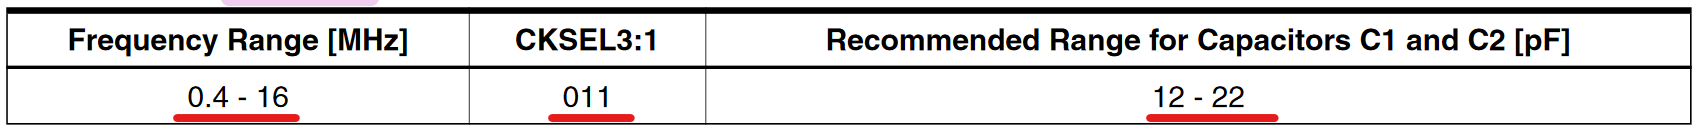
\includegraphics[width=0.7\textwidth]{graphics/Tabelle_Crystal}
	\caption{Tabelle Frequenzbereich Crystal Oszillator.}
	\label{fig:Tabelle_Crystal}
\end{figure}

\todo{cite: Datenblatt Atmega 2560, Seite 43}

\newpage

\begin{figure}[h!]
	\centering
	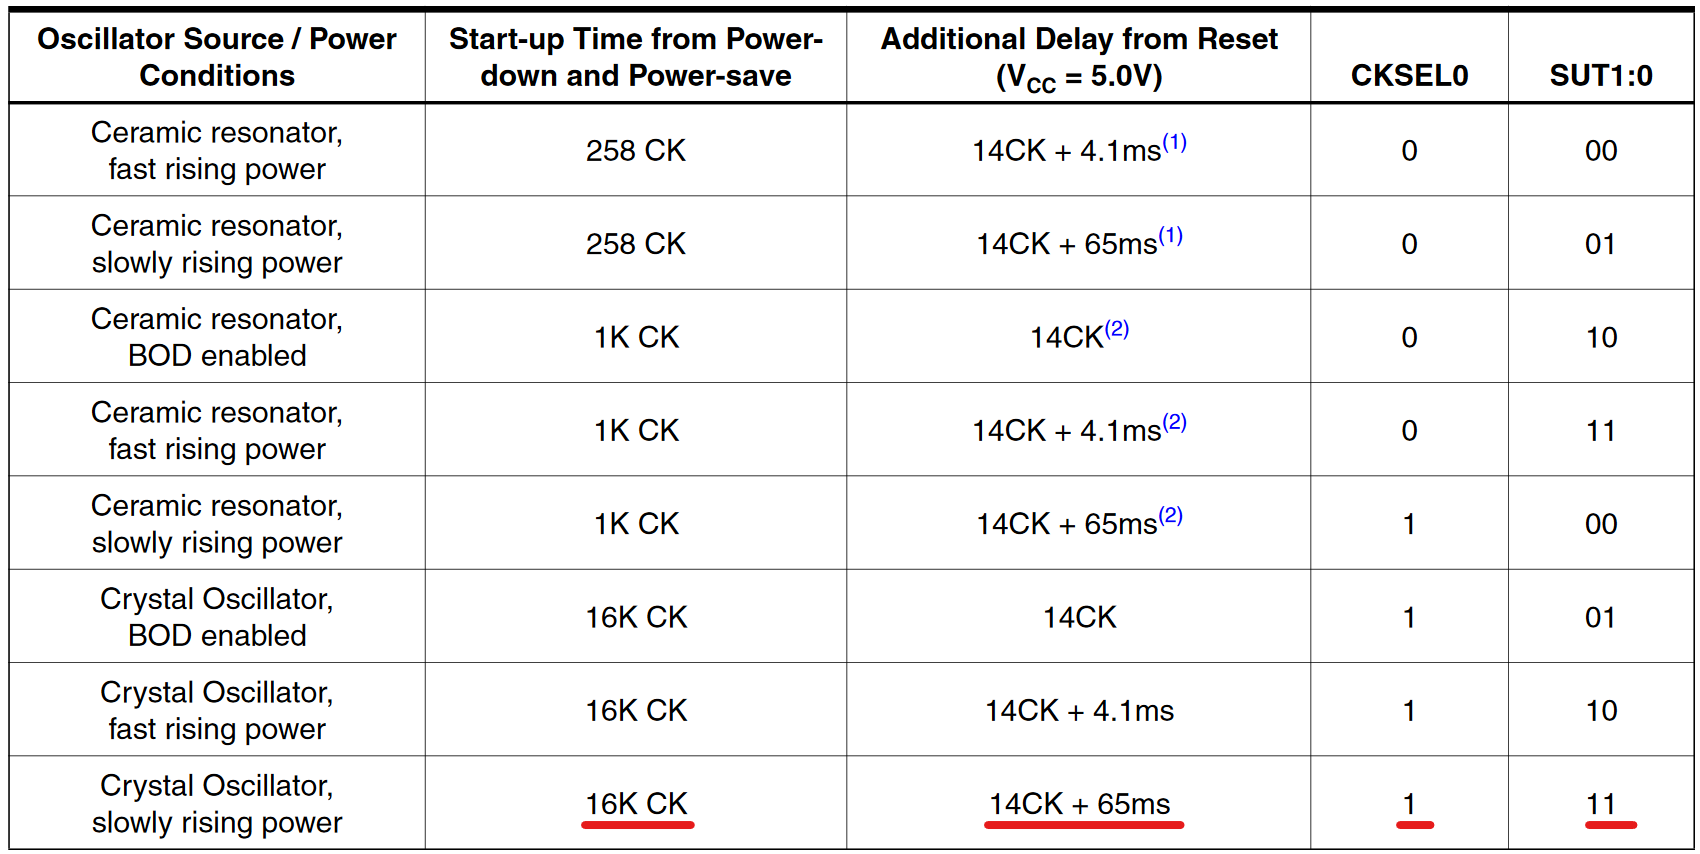
\includegraphics[width=0.7\textwidth]{graphics/Tabelle_Crystal2}
	\caption{Tabelle Aufstartzeit.}
	\label{fig:Tabelle_Crystal2}
\end{figure}

\todo{cite: Datenblatt Atmega 2560, Seite 43}

\subsection{Bootloader-Speicherplatz}\label{Appendix:Bootloader-Speicherplatz}

\begin{figure}[h!]
	\centering
	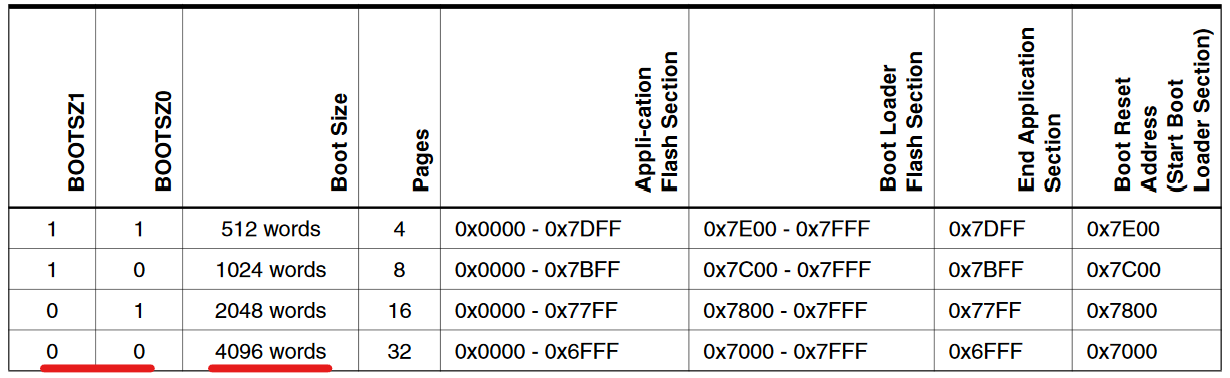
\includegraphics[width=0.7\textwidth]{graphics/Tabelle_Bootloader}
	\caption{Tabelle Bootloader Speicherplatz.}
	\label{fig:Tabelle_Bootloader}
\end{figure}

\todo{cite: Datenblatt Atmega 2560, Seite 320}

\subsection{Memory-Lock Bootloader}

\begin{figure}[h!]
	\centering
	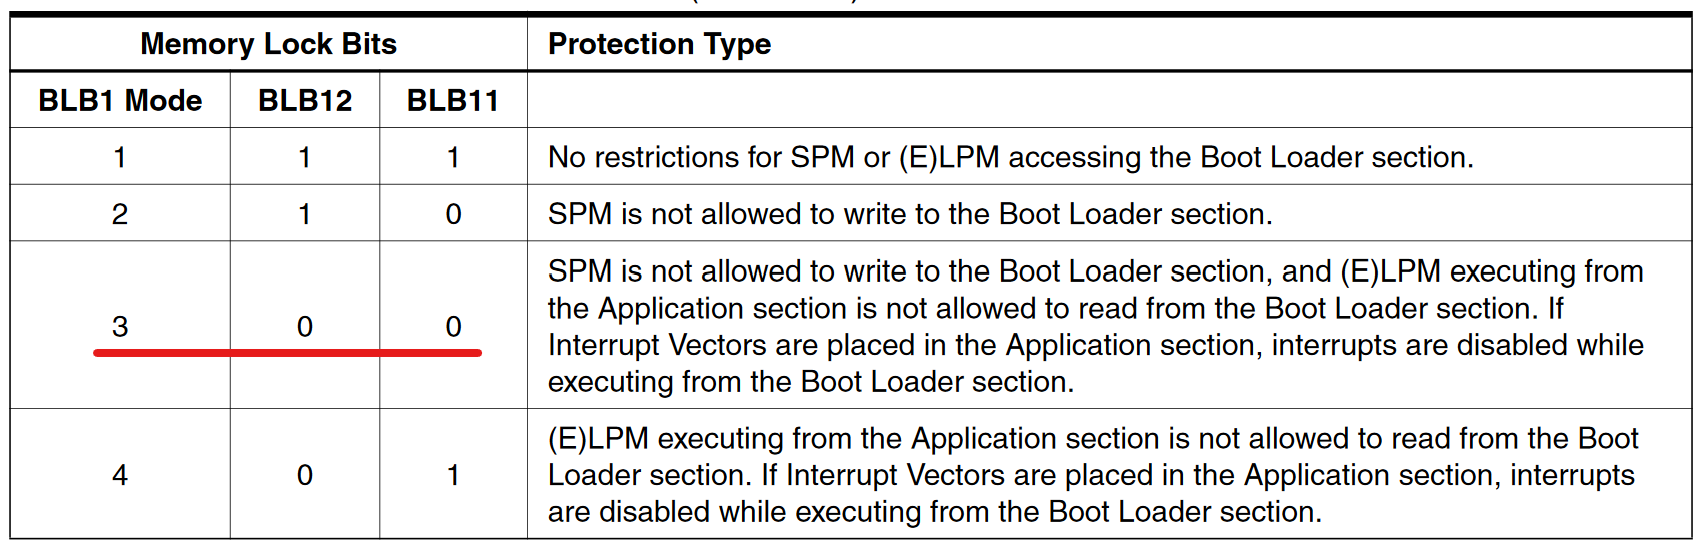
\includegraphics[width=0.7\textwidth]{graphics/Tabelle_Memory_Lock}
	\caption{Tabelle Memory Lock.}
	\label{fig:Tabelle_Memory_Lock}
\end{figure}

\todo{cite: Datenblatt Atmega 2560, Seite 326}

\newpage

\section{Atmel Studio}\label{Appendix:Atmel_Studio}

\subsection{Fuse Bits}

\begin{figure}[h!]
	\centering
	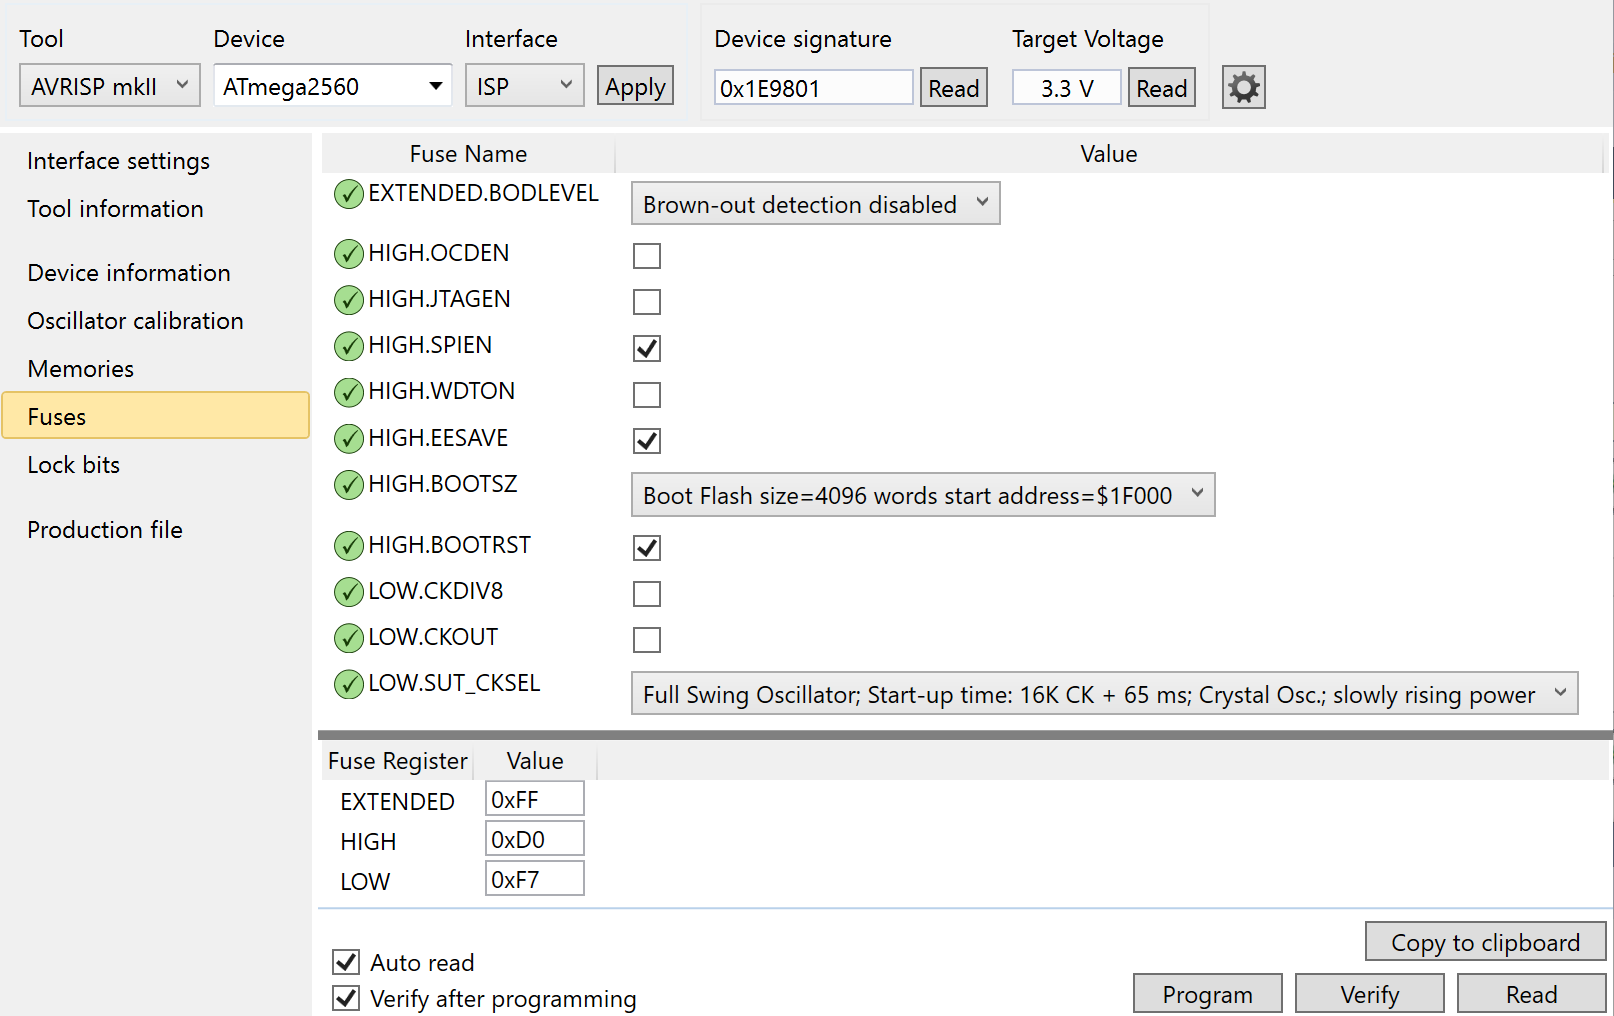
\includegraphics[width=\textwidth]{graphics/AtmelStudio_Fuses}
	\caption{Fuse-Bits Atmega2560.}
	\label{fig:AtmelStudio_Fuses}
\end{figure}

\subsection{Lock Bits}

\begin{figure}[h!]
	\centering
	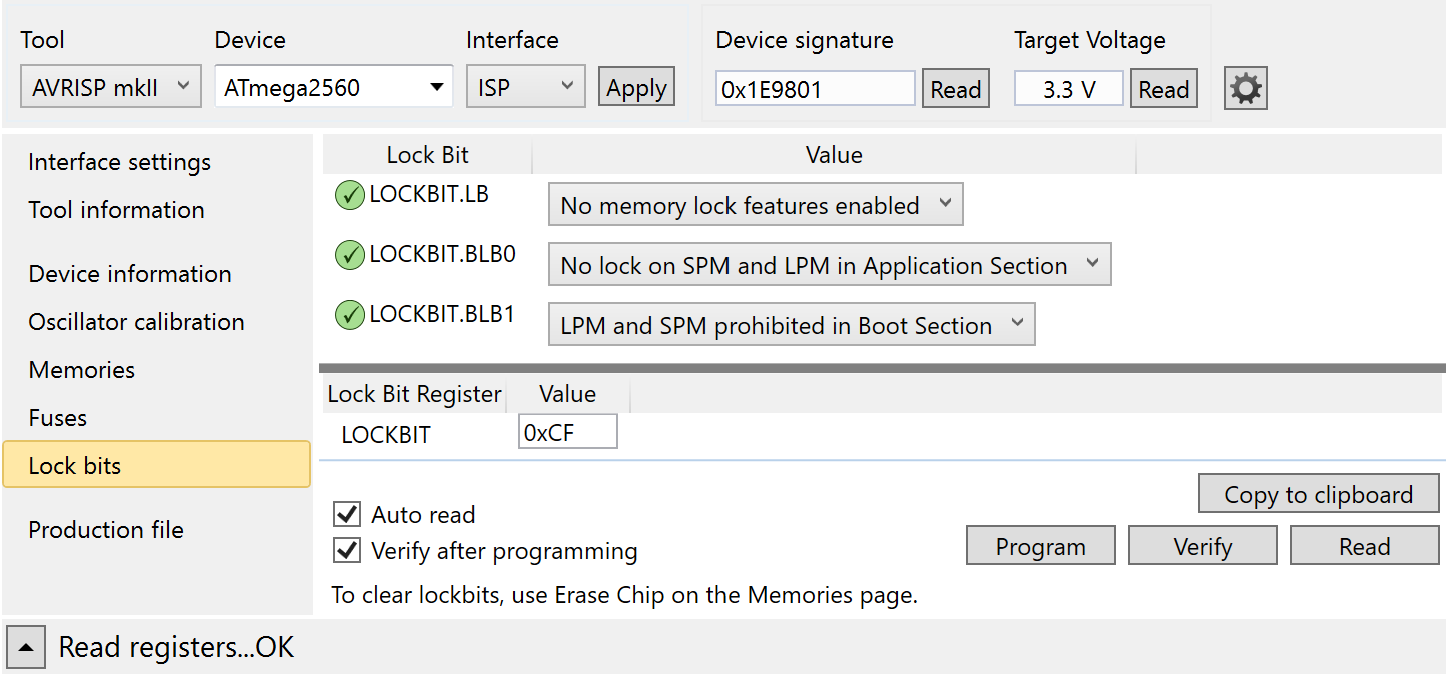
\includegraphics[width=\textwidth]{graphics/AtmelStudio_Locks}
	\caption{Lock-Bits Atmega2560.}
	\label{fig:AtmelStudio_Locks}
\end{figure}
\newpage
\subsection{Einbinden AVRdude und stk500v2 (wiring)}

\begin{figure}[h!]
	\centering
	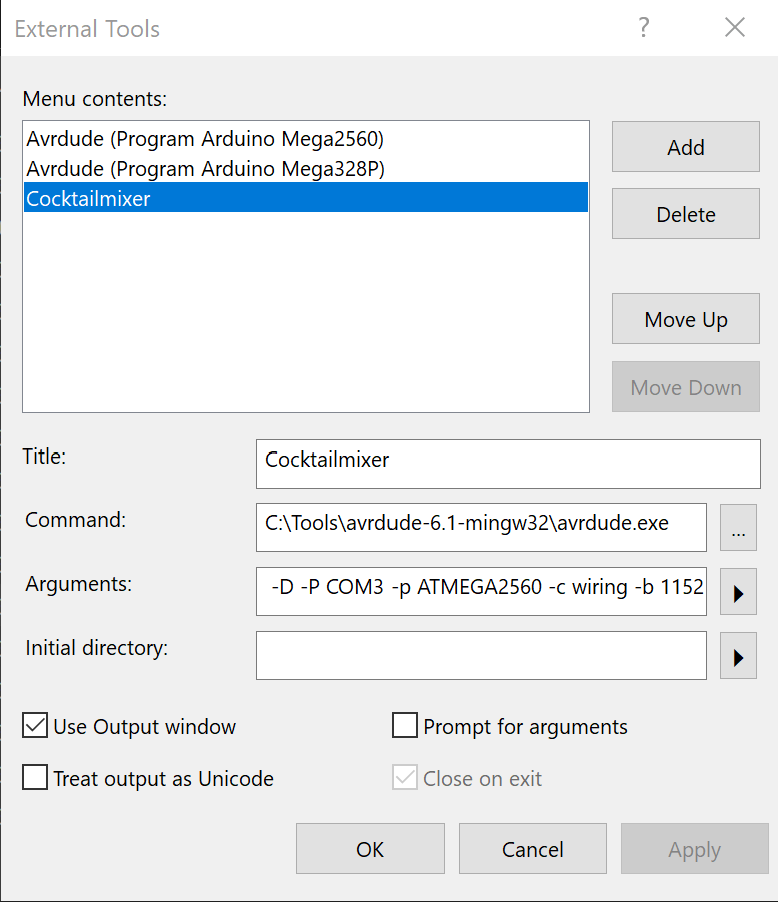
\includegraphics[width=0.5\textwidth]{graphics/AtmelStudio_External_Tools}
	\caption{External Tools Atmega2560.}
	\label{fig:AtmelStudio_Locks}
\end{figure}

\subsection{Bootloader ''Brennen''}

\begin{figure}[h!]
	\centering
	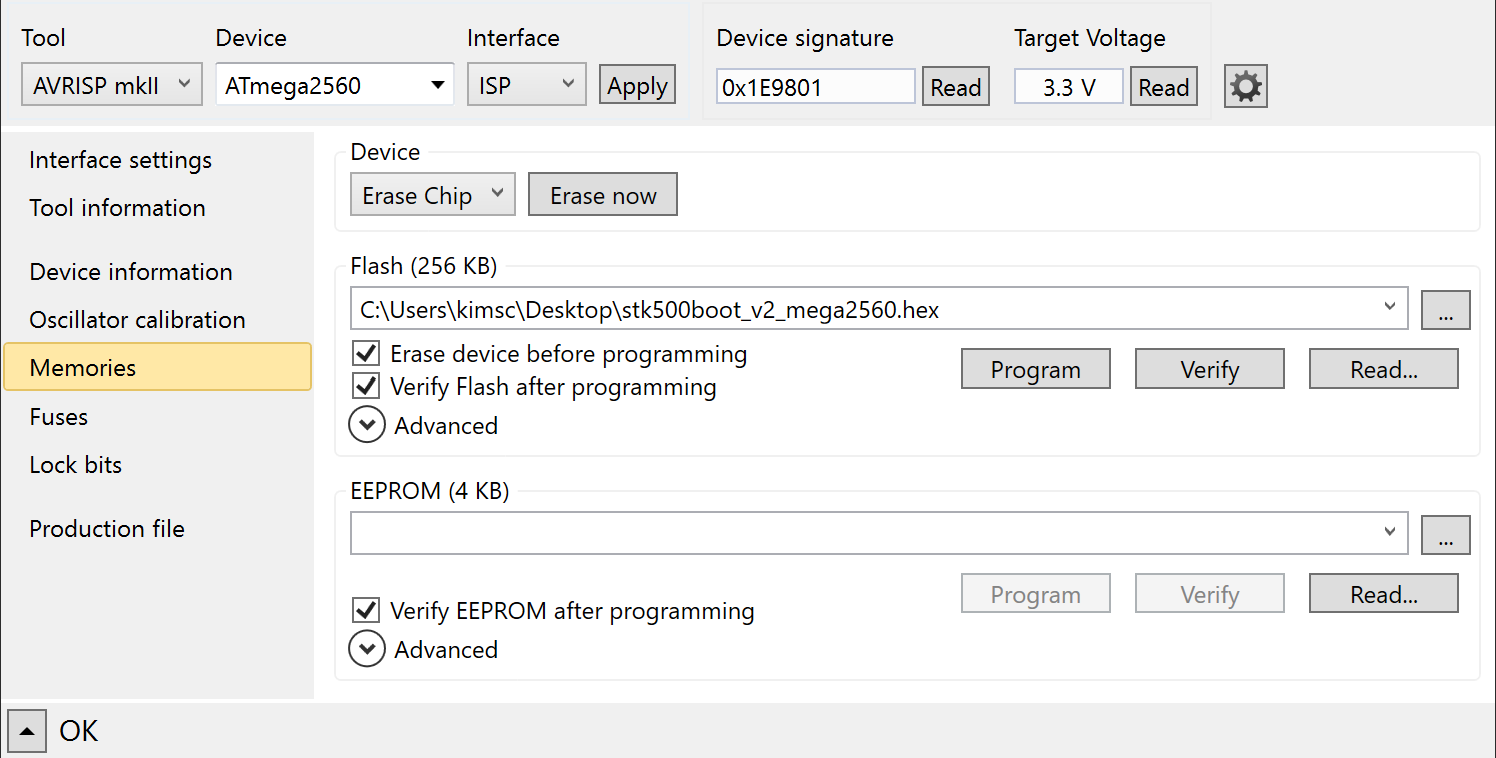
\includegraphics[width=\textwidth]{graphics/AtmelStudio_Program_Bootloader}
	\caption{Bootloader brennen.}
	\label{fig:AtmelStudio_Program_Bootloader}
\end{figure}

\end{appendix}